\chapter{Planificación}

\section{Fases y entregas}

\subsection{Fases}

Como este va a ser un proyecto que ya cuenta con un trabajo previo realizado, la fase inicial de gestión va a ser muy breve
porque se parte de que ya se han realizado varias reuniones y el proyecto está parcialmente funcionando, por lo que no se parte
de cero, es una ampliación de un proyecto inicial.

\begin{itemize}
  \item \textbf{Fase 0:} Gestión del proyecto
  \item \textbf{Fase 1:} Análisis del entorno
  \item \textbf{Fase 2:} Planificación
  \item \textbf{Fase 3:} Desarrollo técnico
\end{itemize}

\subsection{Lista de entregas}

Se harán una serie de breves informes sobre el contenido de cada una de las fases de planificación del proyecto.

\begin{itemize}
  \item \textbf{Fase 0:} Gestión del proyecto
  \begin{itemize}
    \item Descripción: Se realizarán reuniones para concretar los objetivos del proyecto y el desarrollo necesario para 
    cumplirlo.
    \item Tipo: informe.
  \end{itemize}
  \item \textbf{Fase 1:} Especificación del proyecto.
  \begin{itemize}
    \item Descripción: Se establecen los criterios a cumplir para que el desarrollo del proyecto se considere exitoso.
    \item Tipo: informe.
  \end{itemize}
  \item \textbf{Fase 2:} Planificación.
  \begin{itemize}
    \item Descripción: Se desarrolla la documentación con toda la planificación del desarrollo del proyecto indicando aspectos
    como la lista de actividades a realizar, la metodología de trabajo a seguir o las herramientas seleccionadas.
    \item Tipo: informe.
  \end{itemize}
  \item \textbf{Fase 3:} Desarrollo técnico
  \begin{itemize}
    \item Descripción: Implementación del software necesario para cumplir los objetivos, pasando por sus diferentes fases: 
    análisis, diseño, implementación, pruebas. También se realizará una documentación explicativa sobre funcionamiento del 
    mismo.
    \item Tipo: informe.
  \end{itemize}
\end{itemize}

\section{Estructura de Descomposición del Trabajo}

El diagrama de Estructura de Descomposición del Trabajo (figura 3.1) es una descomposición jerárquica de las diferentes fases y 
entregas en las que está planificado el proyecto.

\begin{figure}[htb]
  \begin{center}
  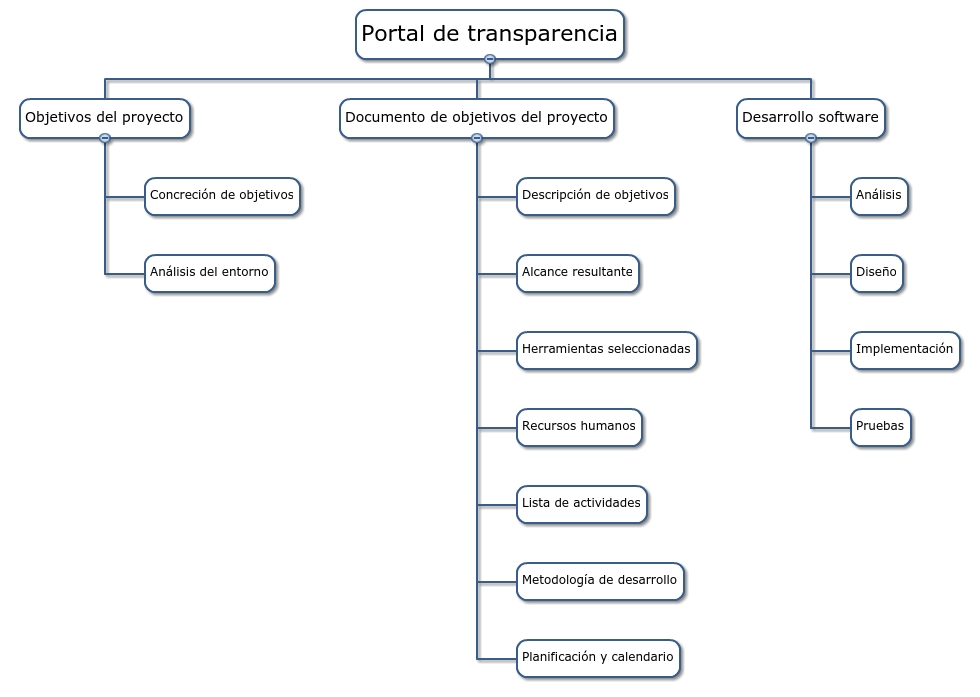
\includegraphics[width=1\textwidth]{imagenes/edt.png}
  \end{center}
  \caption[EDT]{Diagramas Estructura de Descomposición del Trabajo}
\end{figure}

\section{Lista de actividades}

\section{Recursos humanos}

\section{Metodología de desarrollo}

\section{Herramientas seleccionadas}

\section{Temporización}
